\documentclass{beamer}
\usetheme{metropolis}

\usepackage{amsmath, amssymb, amsthm}
\usepackage{cite, graphicx, latexcolors}
\usepackage{ragged2e, microtype}
\usepackage{url, parskip, hyperref}
\usepackage{array, tikz, flowchart}
\usepackage[dvipsnames]{xcolor}

\hypersetup{colorlinks=true,}
\setbeamercolor{title}{fg=orange}

\usetikzlibrary{arrows.meta, calc, chains, quotes, positioning, shapes.geometric}
\tikzset{FlowChart/.style={
    node distance = 5mm and 10mm,
    start chain = A going right,
    base/.style = {draw, minimum width=16mm, minimum height=19mm, align=center, on chain=A, text width=4cm},
    process/.style = {base},
    rounded/.style = {base, rounded corners},
    every edge quotes/.style = {auto=right}
}}

\title[NMPC Implementation]{
    \textbf{
        Implementation of Nonlinear MPC \\
        with Stoch 4 (or) Biped robot
    }
}
\subtitle[Presentation]{\textcolor{mediumpersianblue}{
        \textbf{FoR Project Presentation - 1} \\
    }}
\author[BRAMA]{%
    Team-5 BRAMA
}
\institute[IISc]{    
    Robert Bosch Centre for Cyber Physical Systems,\\
    Indian Institute of Science
}
\date{\today}


\begin{document}


% \section*{Titlepage}
\begin{frame}\titlepage\end{frame}


% \section*{Outline}
\begin{frame}{Outline}
    \begin{enumerate}
        \item Introduction
        \item Literature Survey
        \item Motivation
        \item Implementation strategy
        \item Project Timeline
    \end{enumerate}
\end{frame}


% \section{Introduction}
\begin{frame}{Introduction}
    \begin{enumerate}
        \item Model Predictive Control (MPC)
    \end{enumerate}
\end{frame}\normalfont


\begin{frame}{Literature Survey}
\scriptsize
    \centering
    \begin{table}[ht]
        \resizebox{\textwidth}{!}{
            \begin{tabular}{|>{\centering\arraybackslash}p{2.5cm}|>{\centering\arraybackslash}p{3.0cm}|>{\centering\arraybackslash}p{3.5cm}|>{\centering\arraybackslash}p{5.0cm}|}
                \hline
                \textbf{Title} & \textbf{Authors} & \textbf{Objectives} & \textbf{Key Takeaways} \\
                \hline
                Online Planning for Autonomous Running Jumps Over Obstacles in High-Speed Quadrupeds & Hae-Won Park, Patrick M. Wensing, and Sangbae Kim Department of Mechanical Engineering, MIT, Cambridge, MA, 02139 
 & Presents a novel control framework for quadrupedal robots, enabling dynamic running jumps over obstacles through model predictive control and constrained nonlinear optimization. & Introduces a model predictive control (MPC) framework for dynamic jumping in quadrupeds. \\
                \hline
                Successive Linearization NMPC for a Class of
Stochastic Nonlinear Systems & Mark Cannon, Desmond Ng, and Basil Kouvaritakis &  The proposed method is designed for nonlinear systems with stochastic disturbance &  Can be referred for successive linearization\\
                \hline
                 Variation-Based Linearization of Nonlinear
Systems Evolving on SO(3) and S^2 & Guofam Wu and Koushil Sreenath & Propose a variation-based method to linearize the nonlinear dynamics of robotic systems, whose configuration spaces contain the manifolds S2 and SO(3), along dynamically feasible reference trajectories. & This paper has presented a variation-based method to linearize a nonlinear system, whose dynamics evolve on com-
plex manifolds that contain SO(3) and S2 , along a desired reference trajectory. \\
                \hline
            \end{tabular}
        }
    \end{table}
\end{frame}

\begin{frame}{Literature Survey}
\scriptsize
    \centering
    \begin{table}[ht]
        \resizebox{\textwidth}{!}{
            \begin{tabular}{|>{\centering\arraybackslash}p{2.5cm}|>{\centering\arraybackslash}p{3.0cm}|>{\centering\arraybackslash}p{3.5cm}|>{\centering\arraybackslash}p{5.0cm}|}
                \hline
                \textbf{Title} & \textbf{Authors} & \textbf{Objectives} & \textbf{Key Takeaways} \\
                \hline
                Real-time Model Predictive Control for Versatile Dynamic Motions in
Quadrupedal Robots & Yanran Ding, Abhishek Pandala, and Hae-Won Park & This paper presents a new Model Predictive
Control (MPC) framework for controlling various dynamic
movements of a quadrupedal robot.  & Presents a Model Predictive Control
framework to control various kinds of dynamic maneuvers in
3D space. By directly using linearized models with rotation
matrices, our method could avoid issues arising from use of
local coordinates including singularities (Euler angles) and
unwinding issues (quaternion). Along with this linearization,
the choice of error function on body orientation enables a
QP formulation, which could be efficiently solved to achieve
real-time execution. \\
                \hline
                &  &  &  \\
                \hline
                 &  &  & \\
                \hline
            \end{tabular}
        }
    \end{table}
\end{frame}


\begin{frame}{Motivation}
    \begin{enumerate}
        \item Linearize single RBD rotations matrices \textbf{without resorting to parametrization}
        \item Avoid issues arising from using \textbf{local coordinates}\\
            \textit{Euler angles:} Have singularity issues\\
            \textit{Quaternions:} Unwinding issues
        \item Enable a \textit{QP formulation} for \textbf{real-time execution} using a linearization  technique and use of a configuration error function on $SO(3)$
        \item Development of a \textbf{singularity-free MPC formulation} with consistent performance even when executing motions that involve complex 3D rotations
    \end{enumerate}
\end{frame}


\begin{frame}{Overview}
    \resizebox{\textwidth}{!}{%
    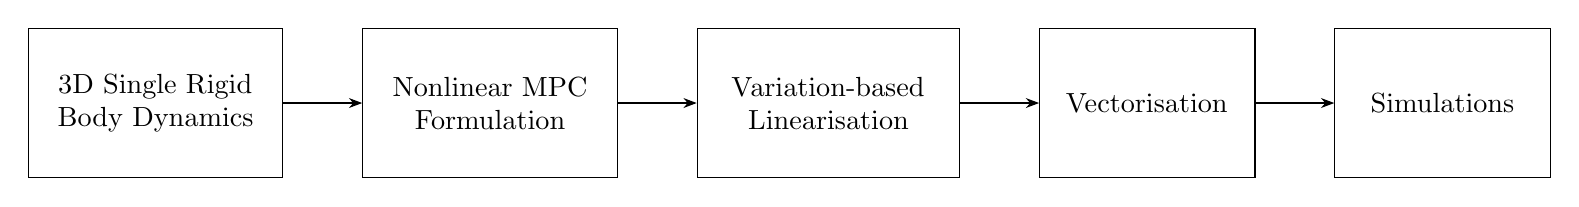
\begin{tikzpicture}[FlowChart]
        \node [process, text width=3cm] {
            3D Single Rigid Body Dynamics
        };
        \node [process, text width=3cm] {
            Nonlinear MPC Formulation
        };
        \node [process, text width=3.1cm] {
            Variation-based Linearisation
        };
        \node [process, text width=2.5cm] {
            Vectorisation
        };
        \node [process, text width=2.5cm] {
            Simulations
        };
    
        \draw [arrows=-Stealth]
        (A-1) edge (A-2)
        (A-2) edge (A-3)
        (A-3) edge (A-4)
        (A-4) edge (A-5);
    \end{tikzpicture}
}


    \setlength{\itemsep}{1em}
    \setlength{\parskip}{2pt} 
    \begin{enumerate}\small
        \item Template model
            \begin{enumerate}\scriptsize
                \item 3D Single Rigid Body Dynamics
                \item Global coordinate frame for rotations
            \end{enumerate}
        \item Nonlinear MPC formulation
            \begin{enumerate}\scriptsize
                \item Non-linear terms for rotations in state space model
                \item Formulate the NMPC as a constrained optimisation problem
            \end{enumerate}
        \item Variation-based Linearisation
            \begin{enumerate}\scriptsize
                \item Succesive Linearisation
            \end{enumerate}
        \item Vectorisation
            \begin{enumerate}\scriptsize
                \item Using Kronecker products
            \end{enumerate}
        \item Simulations
            \begin{enumerate}\scriptsize
                \item Different walking styles
            \end{enumerate}
    \end{enumerate}
    
\end{frame}


\begin{frame}{Project Timeline}
    \scriptsize
\centering
\begin{table}[ht]
    \resizebox{\textwidth}{!}{
        \begin{tabular}{|>{\centering\arraybackslash}p{1.2cm}|>{\centering\arraybackslash}p{3.5cm}|>{\centering\arraybackslash}p{5.5cm}|}
            \hline
            \textbf{Week} & \textbf{Objective}                                  & \textbf{Key Deliverables}                                                  \\
            \hline
            \textbf{1}    & \textbf{Initial Research}& Literature review,  Understanding the model\\
            \hline
            \textbf{2}    & \textbf{Preliminary Model Implementation}& Implementation in Python \\
            \hline
            \textbf{3}    & \textbf{Final Model Implementation}& Implementation in C++ (With a Python interface)\\
            \hline
            \textbf{4}    & \textbf{Simulation}& Simulation in Gazebo\\
            \hline
            \textbf{5}    & \textbf{Testing and Validation}& Validation of our implementation using Gazebo simulation for different walking styles\\
            \hline
            \textbf{6}    & \textbf{Report}& Preparation of Report and additional objectives (if any)\\
            \hline
            \textbf{7}    & \textbf{Final Presentation}& Final report, presentation slides, demo videos                             \\
            \hline
        \end{tabular}
    }
\end{table}

\end{frame}


\begin{frame}
    \LARGE{Thank You!}
\end{frame}


\end{document}
